% 
\documentclass[a4paper,10pt]{article}
\usepackage[utf8x]{inputenc}
\usepackage[OT1]{fontenc}
\usepackage{hyperref}
\usepackage{Sweave}
\usepackage{graphicx}
\usepackage{color}
\graphicspath{figures/}
\usepackage{float}
\usepackage{wrapfig}
\usepackage{subfigure}
%% Package to linebreak URLs in a sane manner.
\usepackage{url}
%% Define a new 'smallurl' style for the package that will use a smaller font.
\makeatletter
\def\url@smallurlstyle{%
  \@ifundefined{selectfont}{\def\UrlFont{\sf}}{\def\UrlFont{\small\ttfamily}}}
\makeatother
%% Now actually use the newly defined style.
\urlstyle{smallurl}
%% Define 'tinyurl' style for even smaller URLs (such as in tables)
\makeatletter
\def\url@tinyurlstyle{%
  \@ifundefined{selectfont}{\def\UrlFont{\sf}}{\def\UrlFont{\scriptsize\ttfamily}}}
\makeatother
%% Make margins less ridiculous
\usepackage{fullpage}
%% Make URLs clickable
%\usepackage[colorlinks, bookmarks=false]{hyperref}
%\usepackage[colorlinks, bookmarks=true]{hyperref}
%% Since I'm using the LaTeX Makefile that uses dvips, I need this
%% package to make URLs break nicely
\usepackage{breakurl}
\usepackage{todonotes}
\usepackage{amsmath,amsfonts}
\numberwithin{equation}{subsection}
%%\usepackage{nonfloat}
\usepackage{bbm}
\usepackage{setspace}
\onehalfspacing
\usepackage{tabularx}

%
%
%
\usepackage{listings}
\usepackage{courier}
\lstset{
         basicstyle=\footnotesize\ttfamily, % Standardschrift
         %numbers=left,               % Ort der Zeilennummern
         numberstyle=\tiny,          % Stil der Zeilennummern
         stepnumber=2,               % Abstand zwischen den Zeilennummern
         numbersep=5pt,              % Abstand der Nummern zum Text
         tabsize=2,                  % Groesse von Tabs
         extendedchars=true,         %
         breaklines=true,            % Zeilen werden Umgebrochen
         keywordstyle=\color{red},
    		frame=b,         
 %        keywordstyle=[1]\textbf,    % Stil der Keywords
 %        keywordstyle=[2]\textbf,    %
 %        keywordstyle=[3]\textbf,    %
 %        keywordstyle=[4]\textbf,   \sqrt{\sqrt{}} %
         stringstyle=\color{white}\ttfamily, % Farbe der String
         showspaces=false,           % Leerzeichen anzeigen ?
         showtabs=false,             % Tabs anzeigen ?
         xleftmargin=17pt,
         framexleftmargin=18pt,
         framexrightmargin=6pt,
         framexbottommargin=4pt,
         %backgroundcolor=\color{lightgray},
         showstringspaces=false      % Leerzeichen in Strings anzeigen ?        
 }
 \lstloadlanguages{% Check Dokumentation for further languages ...
         %[Visual]Basic
         %Pascal
         %C
         %C++
         %XML
         %HTML
         Java
 }
%\DeclareCaptionFont{blue}{\color{blue}} 
%\captionsetup[lstlisting]{singlelinecheck=false, labelfont={blue}, textfont={blue}}
\usepackage{caption}
\DeclareCaptionFont{white}{\color{white}}
\DeclareCaptionFormat{listing}{\colorbox[cmyk]{0.43, 0.35, 0.35,0.01}{\parbox{\textwidth}{\hspace{15pt}#1#2#3}}}
\captionsetup[lstlisting]{format=listing,labelfont=white,textfont=white, singlelinecheck=false, margin=0pt, font={bf,footnotesize}}
%
%

\begin{document}

\title{Mining of Android SCM}
\author{Pavel Senin}

\maketitle

\begin{abstract}
MSR (mining software repositories) challenge is an annual competition for researchers working in the area of
software engineering to demonstrate their tools and approaches for discovering actionable information within
software artifacts trails. Android OS was selected as the research subject for 2012 MSR Challenge. 
Here I report an application of Software Trajectory toolkit to the challenge data along with discussing my findings.
(I will put a summary of findings here later)
\end{abstract}

\section{Introduction}
The research field of Mining Software Repositories (MSR) is focused on analyzes of the rich 
data available in software repositories. The immediate goal of such research is to infer interesting 
and actionable information about software systems and projects. While there are multiple scientific 
events where researchers working in the field meet, the Mining Software Repositories 
conference considered to be the major one. The current 2012 MSR conference is a 9th such event
and is collocated with ICSE -the International Conference on Software Engineering.
Along with research track, since 2006 MSR Conference agenda includes the Mining Challenge where 
researchers demonstrate application of their tools to the selected repository mining problem. This
year Android platform was selected for the challenge.

\section{Android OS}
``Android is an open-source software stack for mobile phones and other devices'' as it said 
at its home website, \url{http://source.android.com/}: 

The development of Android OS was started by Android Inc. - a small startup company - which was purchased by Google 
in 2005. Later, in November 2007, the Open Handset Alliance, a consortium of 84 companies, announced 
the availability of the Android Software Development Kit (SDK). This open Open Handset Alliance was formed 
of hardware, software, and telecommunication companies (including Intel, HTC, ARM, Samsung and Motorola)
and its creation was devoted to advancing of open standards for mobile devices. 

As with any other open-source system, the Android OS code is open and released under the Apache License.
As promised, it is a complete mobile platform built on the monolithic Linux 2.6 kernel. 
The Android platform provides developers with an SDK consisting of a set of development tools, 
debugger and a true device emulator. To speed-up development there are an Eclipse plugin, 
a set of libraries, a multimedia user interface, and a core set of phone and mobile applications. 
The Android application model alleviates the cost of software development by 
allowing extending, replacing, and reusing of existing software components. 
The Dalvik virtual machine, which is the part of Android distribution, provides a way to 
maximize application portability, performance and security. 
Android OS allows true application multitasking, provides rich user 
notifications and customizable home screens with resizable widgets. 
Latest, 4.0 version of Android System provides streaming voice recognition.
\begin{wrapfigure}{l}{0.5\textwidth}
    \begin{center}
   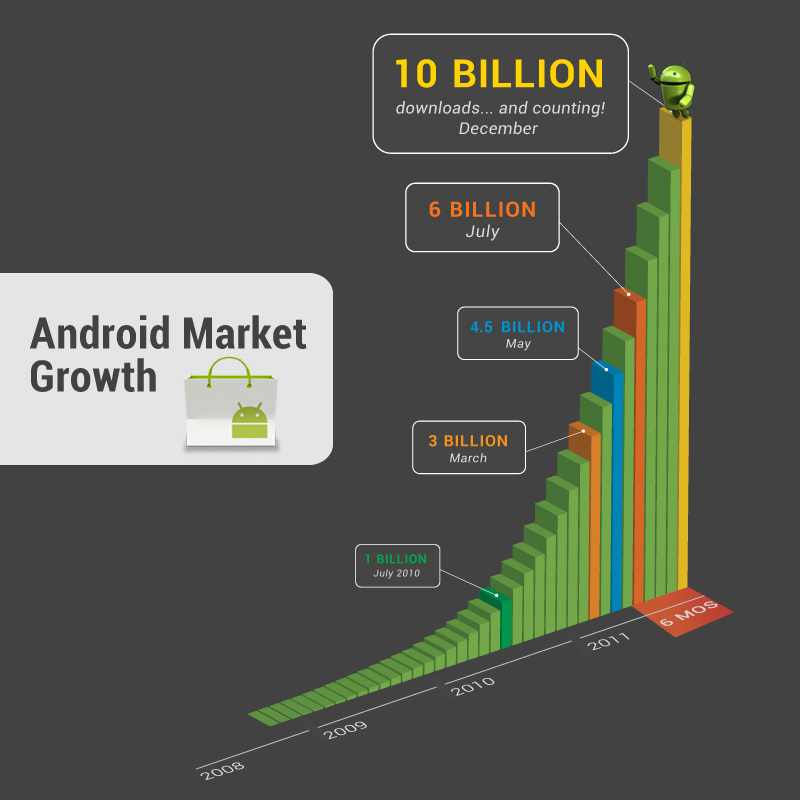
\includegraphics[scale=0.3,width=0.48\textwidth]{figures/graph_only_3.png}
   \end{center}
   \caption{The Android store downloads timeline.}
   \label{fig:android_downloads}
\end{wrapfigure}

Currently, the Android Open Source Project (AOSP) is led by Google and includes not only the 
original members of OHA but many other companies. The role of AOSP is to maintain and develop 
Android.

Including first beta, there were 10 major releases of Android as well as a number of intermediate 
releases. All releases prior to 2.0 were for mobile phones exclusively. Since 2.0 release 
Android OS is a tablet-oriented operating system. Most of the mobile devices at market use 
2.x version of Android. The 3.0 release, Honeycomb, does not officially run on phones; 
the latest 4.0 release, Ice Cream Sandwich, runs on all mobile devices.

In Q3, 2011 (November 15, 2011) Android officially become the most popular OS for newly sold mobile 
devices. In December 2011 there were registered 10 billions of downloads from Android store called
Android Marketplace. 

Two XML files containing change and bug report 
data were offered to participants to uncover interesting facts related to the Android platform.

\lstset{label=changeXSDFragment,caption=List of metadata provided by change trail XML (fragment) }
\begin{lstlisting}
 <xs:element name="change">
    <xs:complexType>
      <xs:sequence>
        <xs:element ref="project"/>
        <xs:element ref="commit_hash"/>
        <xs:element ref="tree_hash"/>
        <xs:element ref="parent_hashes"/>
        <xs:element ref="author_name"/>
        <xs:element ref="author_e-mail"/>
        <xs:element ref="author_date"/>
        <xs:element ref="commiter_name"/>
        <xs:element ref="commiter_email"/>
        <xs:element ref="committer_date"/>
        <xs:element ref="subject"/>
        <xs:element ref="message"/>
        <xs:element ref="target"/>
      </xs:sequence>
    </xs:complexType>
  </xs:element>
\end{lstlisting}

\section{Research question.}
In this exploratory study I am trying to address an important question - is the SAX-based temporal data
mining methods are capable of discovering recurrent behaviors and do the discovered behaviors reflect 
any interesting and actionable information.

\section{Challenge data.}
Two XML files were offered for the MSR challenge. These files contain the most of the information
obtainable from Google-hosted source code repository (Git) as well as Google-hosted bug and issue
tracking system (Google project hosting). 
The full XSD for both XML files can be found in the Appendix section of this report.
While the issues and comments trail \ref{bugsXSD} provided nearly complete information,
the change trail \ref{changeXSD} provided for a challenge contained only the high-level change information.
The thirteen data fields of the change trail XSD file shown at the fragment Listing \ref{changeXSDFragment}. 
The provided data contains information about revision tree, author and a commiter identification, change
message and affected targets.
Since I am focusing on mining of temporal patterns for inferring recurrent behaviors, I consider 
this provided dataset rather poor since it lacks many of auxiliary change and target information. 
In fact, among relevant to Trajectory toolkit data fields, every timestamped entity of the offered trail
contain only author id and an indication of affected targets (the committer information
is rather useless for trajectory since it could not be trusted due to the nature of git merged commits).   

\subsection{Android SCM facts}
There are 1771667 changes registered in the repository. First change commit to Android repository dates back 
to Monday, January 12th, 1970, 14:46:40, while the last change within the analyzed data set belongs Tuesday, 
June 21st 2011, 12:41:41. The detailed data about changes per project is available in the Appendix Table 
\ref{tab:projects}. I was not able to recover the state of repository as it was parsed into XML, but 
per January, 1, 2012 Android repository contains a total of 26851267 lines of source code in 152225 files. 

\section{Auxiliary information collection and data organization.}
In order to enrich the provided data for recurrent pattern analysis I decided to collect auxiliary 
information for changes. I have created a local mirror of Android OS and by iterating over existing 
commits hashes was able to recover auxiliary data for 68\% of existing commits. The rest 
of changes which is about 32\% of total change information belonging to legacy projects is 
unrecoverable due to the recent changes in Android repository. 

For every recoverable change record I collected a summary of added, modified or deleted files 
as well as a summary about LOC changes: added, modified or deleted lines.

All this information was stored in the Trajectory database backend (since the TrajectoryDB schema
was designed to accommodate change artifact trails from CVS and SVN repositories I have extended
it to accommodate Git change data such as tree hash, commit hash and a commiter identification).
The main tables of TrajectoryDB correspond to entities of change log and issue log; these tables 
accompanied with separate tables for change targets and issue comments as well as tables for
authors, contributors etc. Overall, the TrajectoryDB is normalized and optimized for the fast 
retrieval of change and issue information using SQL language.

\begin{wrapfigure}{l}{0.5\textwidth}
   \begin{center}
   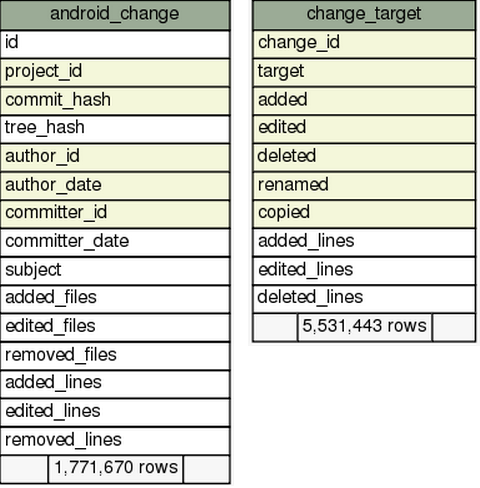
\includegraphics[scale=0.4,width=0.5\textwidth]{figures/schema-change-fragment.png}
   \end{center}
   \caption{The Trajectory DB schema fragment. Change and target tables shown.}
   \label{fig:schema_change_fragment}
\end{wrapfigure}

\section{Threats to Validity}
Before discussing the mining methodology and my findings I discuss several threats to validity 
of this research and how I have addressed them. These include general threats to construct 
validity, external validity, and specific threats to my particular methodology including 
repository threats, recall and precision. 

\subsection{General threats.}
Construct validity requires that Trajectory must correctly identify authors and their activity.
The threat to the construct validity comes from the shortcomings of both: the repository data and
the Trajectory toolkit. First of all, it is hard to access how much of the contributor's activity 
devoted to the project is actually captured within the artifact trails. Certainly, it is 
insufficient to look only on the this data for drawing any general conclusion about contributors 
behavior or about all or part of Android operating system. Moreover the approximation and reduction 
of information within Trajectory workflow creates further difficulties for any assertion. Thus,
I do not claim external validity and as in any other exploratory and characteristic in nature 
study this work should be considered together with evaluation methodology.

\subsection{Repository data threats.}
The Android OS developers using Git as the SCM system. Git is a distributed revision control system 
with an emphasis on speed. Git keeps all the history on the local machine allowing very fast 
branching and easy repeated merging of branches thus creating multiple trees which deviate from 
mainline (trunk). In my analyzes I ignore Git merge commits which only record metadata about 
integration between different development trees. 

\subsection{Treats due to incompleteness of data.}
The information enclosed for the challenge appears to be partially not reproducible due to the 
changes happened within the Android OS hosting scheme and deletion of some legacy projects.
Based on my own retrieval of the auxiliary data, it is impossible to confirm about 32\% of all
change records found in XML file. This fact implies that in my analyzes I missed some of the 
quantitative change information, however in my opinion there is no reason to believe that 
the lack of this data affect behavioral patterns recognition and classification. The reason
for this statement is that the general development behavior doesn't change much between projects.
For example \ldots

\subsection{Threats to commit characteristics.}
Some of the contributors of Android OS commit using several email addresses and some of the 
contributors have a variation in their names thus possessing a threat to author classification.
In order to address this threat I have merged together authors which share the same full name
reducing the authors id set from 11311 names to 8706.

\section{Data curation.}
In order to proceed with patterns mining apply Trajectory framework After the collection of auxiliary data 
The data collected at the previous step was filtered into the separate database table for further analyzes.
The reason to perform this step was the overall amount of merged commits (~35K) as well as the amount of 
commits which lacked the auxiliary data (~581K).

\section{Data reduction and indexing}
SAX indexing depends on the three parameters which are required input. First parameter is
the sliding window, second is the PAA approximation size and third is the SAX Alphabet size.

In this work I have selected three sizes for sliding window: 7 days, 14 days and 30 days. 
These represent an intuitive and logical intervals of a week, two weeks and a month.

For the PAA reduction I choose 3 steps for 7 days window, 5 steps for a weekly interval,
and 7 steps for a monthly window.

Finally the alphabet, I choose 3 letters for weekly window, and 5 letters for bi-weekly and monthly windows.
All these are summarized in the Table \ref{tab:parameters}.

\begin{table}
  \caption{Sliding window, PAA and alphabet size choices.}
  \centering
  \label{tab:parameters}
  \begin{tabularx}{270pt}{ | X | c | c |}
  \hline                       
  Sliding window size & PAA size & Alphabet size \\
  \hline 
    one week (7) & 3 & 3 \\  
    two weeks (14) & 5 & 5 \\ 
    month (30) & 5 & 5 \\ 
  \hline  
  \end{tabularx}
\end{table}

There will be a detailed indexing procedure description

\section{Results}
For application of the Trajectory toolkit I need to select particular projects from the Android OS
project tree \url{https://sites.google.com/a/android.com/opensource/projects}. I have decided to 
select three sub-projects: the one of OS kernels, the Core Android App Framework libraries 
(frameworks\_base) and a bluetooth subsystem components (platform\_external\_bluetooth\_bluez and 
platform\_external\_bluetooth\_glib).

\begin{figure}[htb]
  \centering
  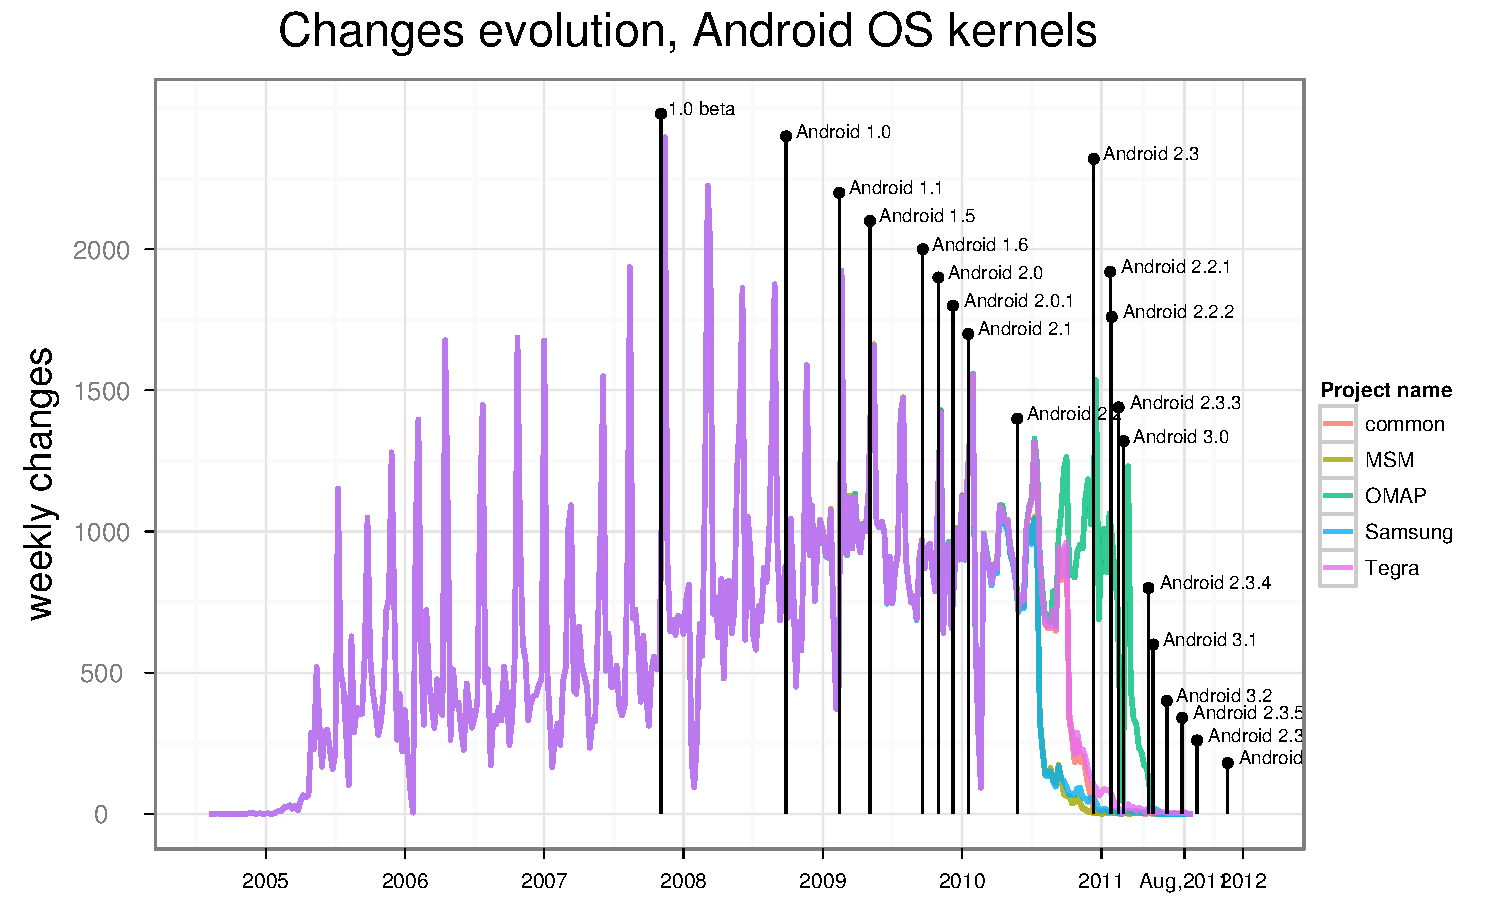
\includegraphics[width=0.9\textwidth]{figures/kernels_changes.pdf}
  \caption{Weekly changes in Android OS kernel sub-projects}
  \label{fig:kernels_changes}
\end{figure}

As Figure \ref{fig:kernels_changes} shows that there is almost no difference in the SCM trails of 
pre-2010 kernels, thus I have arbitrary selected the OMAP-kernel which is a customized 
Linux 2.6 kernel for OMAP-based devices. OMAP is a proprietary system on chips (SoCs) for 
portable and mobile multimedia applications and based on general-purpose ARM architecture 
processor provided by Texas Instruments \url{http://en.wikipedia.org/wiki/OMAP}.

While picking a single project from the kernel sub-projects was a trivial task. The choice of 
other projects was not that easy. If we look at the number of changes and their distribution
in time, picking project randomly could impose the treat of insufficient sample size. By 
looking on the the number of changes and the activity interval I have picked the 
Core Android App Framework \ref{fig:projects_changes} and a bluetooth stack \ref{fig:bluetooth_changes}.

\begin{figure}[htb]
  \centering
  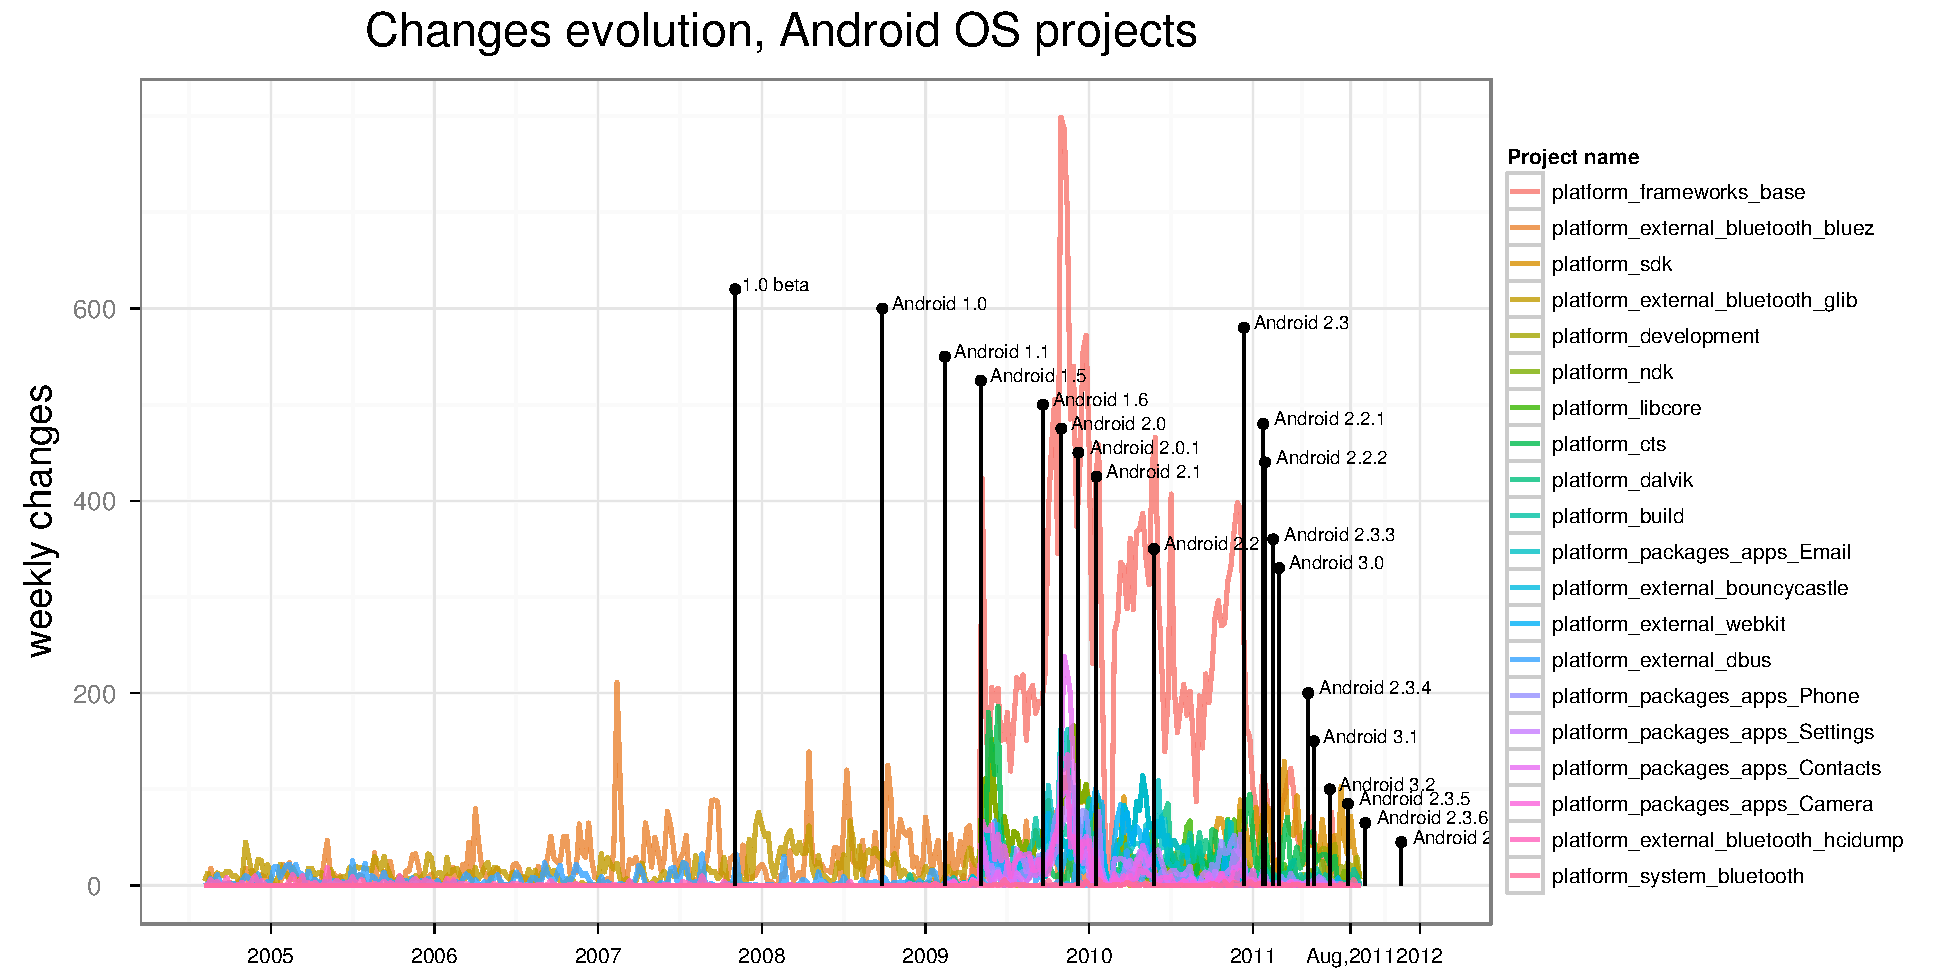
\includegraphics[width=0.9\textwidth]{figures/projects_changes.pdf}
  \caption{Weekly changes in Android OS sub-projects}
  \label{fig:projects_changes}
\end{figure}

By indexing these three trails with Trajectory SAX workflow and successive indexing I obtained
dictionaries of patterns and their occurence frequencies. By using SQL it is fairly easy
to extract the index of patterns for the project, inteval and an author.

\begin{figure}[htb]
  \centering
  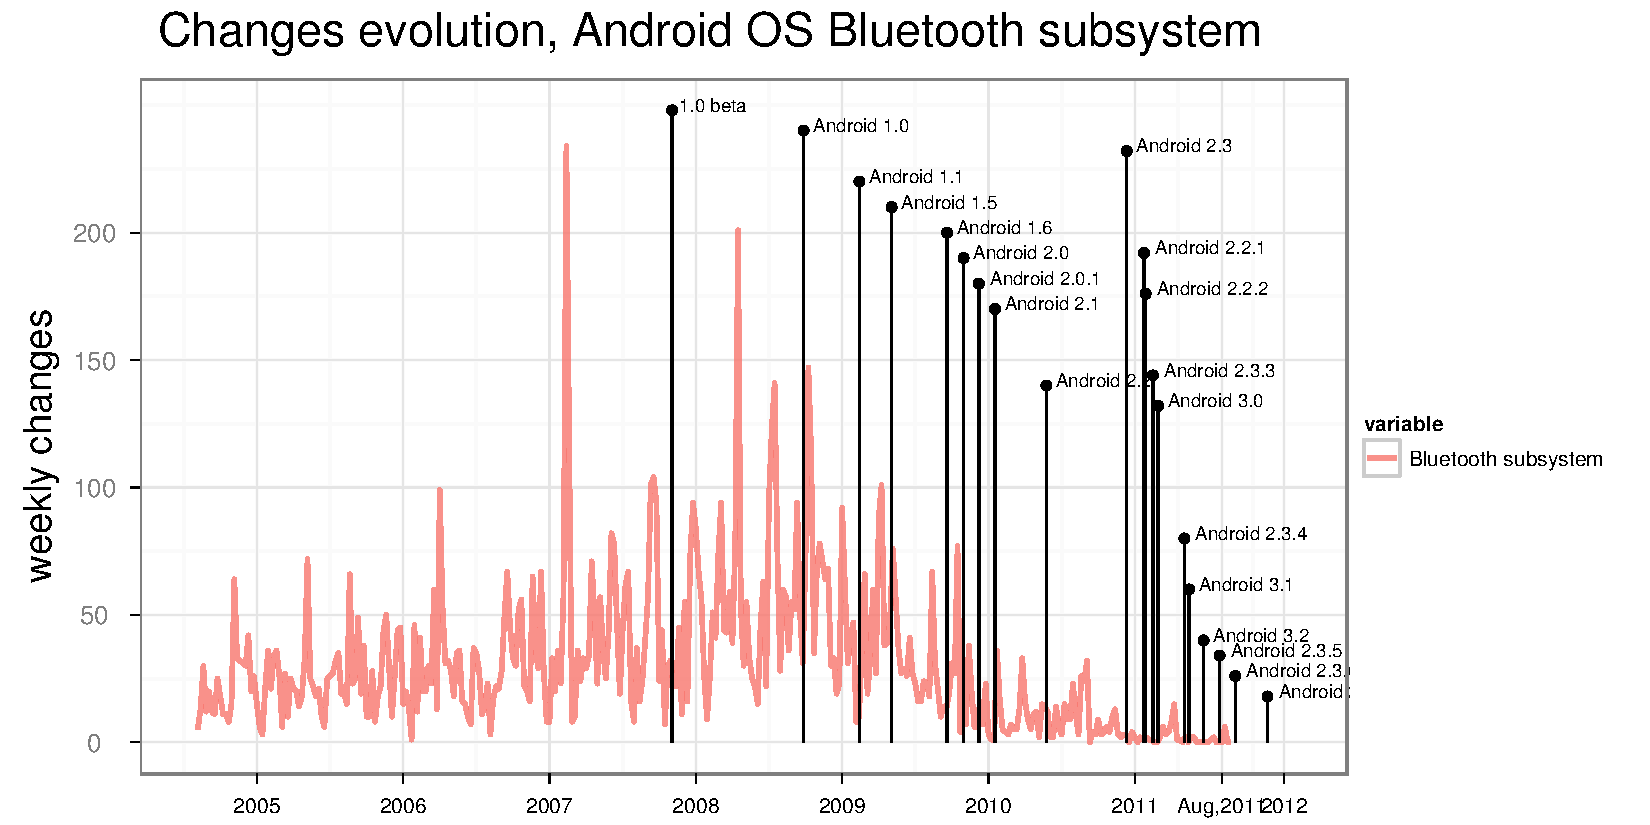
\includegraphics[width=0.9\textwidth]{figures/bluetooth_changes.pdf}
  \caption{Weekly changes in Android OS Bluetooth sub-system.}
  \label{fig:bluetooth_changes}
\end{figure}

\subsection{OMAP kernel pre-release and post-release patterns}
First I looked on the patterns seen within the Android OS release proximity in OMAP kernel
project. The table \ref{tab:omap_weekly} shows sorted by frequency weekly patterns observed
by indexing a stream of changed targets.
\begin{table}
  \caption{OMAP kernel weekly patterns sorted by occurence.}
  \centering
  \label{tab:omap_weekly}
  \begin{tabularx}{450pt}{ | l | X |}
  \hline                       
  Release label & Sorted patterns  \\
  \hline 
  Android 1.0-2M & bbb,cbb,bbc,bcb,ccc,cba,acb,bca,abc,bac,caa,bba,abb,cab,aac,bab,aca,cac,cca,acc\\ 
  Android 1.0-1M & bbb,cbb,bbc,bcb,ccc,bca,cba,abc,acb,bba,caa,aac,abb,bac,cab,bab,aca,acc,cca\\ 
  Android 1.0+1M & bbb,bbc,cbb,bcb,ccc,cba,abc,acb,bca,caa,aac,abb,bba,cab,bac,bab,aca,cac\\ 
  Android 1.1-2M & bbb,bbc,cbb,bcb,ccc,abc,cba,acb,bca,abb,bba,caa,aac,cab,bac,bab,aca,cca\\ 
  Android 1.1-1M & bbb,bbc,cbb,bcb,ccc,cba,bca,abc,acb,caa,cab,bba,aac,abb,bac,bab,aca\\ 
  Android 1.1+1M & bbb,cbb,bbc,bcb,ccc,cba,acb,bca,abc,cab,bac,abb,bba,caa,aac,bab,aca,acc,cca\\ 
  Android 1.5-2M & bbb,bbc,cbb,bcb,ccc,bca,acb,cba,abc,abb,cab,bac,bba,aac,bab,caa,aca,acc,cca\\ 
  Android 1.5-1M & bbb,cbb,bbc,bcb,ccc,cba,bca,acb,abc,caa,bba,abb,aac,bac,cab,bab,aca\\ 
  Android 1.5+1M & bbb,bbc,cbb,bcb,ccc,acb,cba,bca,abc,cab,abb,aac,bac,caa,bba,bab,aca\\ 
  Android 1.6-2M & bbb,bbc,cbb,bcb,ccc,acb,bca,cba,abc,abb,aac,caa,bba,cab,bac,bab,aca\\ 
  Android 1.6-1M & bbb,bbc,cbb,bcb,ccc,bca,acb,cba,abc,bba,abb,aac,caa,cab,bac,bab,aca\\ 
  Android 1.6+1M & bbb,bbc,cbb,bcb,ccc,cba,bca,acb,abc,caa,abb,bac,cab,bba,aac,bab,aca \\
  \hline  
  \end{tabularx}
\end{table}

When SAX minimal bounding distance is applied to these vectors 

\begin{table}
  \caption{OMAP kernel weekly patterns distance matrix.}
  \centering
  \label{tab:omap_weekly_distance}
  \begin{tabularx}{450pt}{ | X | c | c | c | c | c | c | c | c | c | c | c | c |}
  \hline                       
  &  & & & & & & & & & & & \\
  \hline 
Android 1.0-2M & 0.0 & 6.02 & 3.44 & 5.16 & 2.58 & 2.58 & 3.44 & 1.72 & 4.3 & 2.58 & 3.44 & 3.44\\ 
Android 1.0-1M & 6.02 & 0.0 & 5.16 & 4.3 & 0.86 & 4.3 & 2.58 & 0.0 & 2.58 & 5.16 & 4.3 & 3.44\\ 
Android 1.0+1M & 3.44 & 5.16 & 0.0 & 8.6 & 3.44 & 2.58 & 6.02 & 3.44 & 5.16 & 5.16 & 1.72 & 1.72\\ 
Android 1.1-2M & 5.16 & 4.3 & 8.6 & 0.0 & 3.44 & 8.6 & 7.74 & 4.3 & 4.3 & 3.44 & 6.88 & 5.16\\ 
Android 1.1-1M & 2.58 & 0.86 & 3.44 & 3.44 & 0.0 & 2.58 & 4.3 & 0.0 & 5.16 & 6.0 & 6.02 & 2.58\\ 
Android 1.1+1M & 2.58 & 4.3 & 2.58 & 8.6 & 2.58 & 0.0 & 2.58 & 3.44 & 3.44 & 2.58 & 0.0 & 0.0\\ 
Android 1.5-2M & 3.44 & 2.58 & 6.02 & 7.74 & 4.3 & 2.58 & 0.0 & 2.58 & 5.16 & 2.58 & 1.72 & 3.44\\ 
Android 1.5-1M & 1.72 & 0.0 & 3.44 & 4.3 & 0.0 & 3.44 & 2.58 & 0.0 & 1.72 & 5.16 & 2.58 & 2.58\\ 
Android 1.5+1M & 4.3 & 2.58 & 5.16 & 4.3 & 5.16 & 3.44 & 5.16 & 1.72 & 0.0 & 4.3 & 2.58 & 1.72\\ 
Android 1.6-2M & 2.58 & 5.16 & 5.16 & 3.44 & 6.02 & 2.58 & 2.58 & 5.16 & 4.3 & 0.0 & 1.72 & 3.44\\ 
Android 1.6-1M & 3.44 & 4.3 & 1.72 & 6.88 & 6.02 & 0.0 & 1.72 & 2.58 & 2.58 & 1.72 & 0.0 & 0.86\\ 
Android 1.6+1M & 3.44 & 3.44 & 1.72 & 5.16 & 2.58 & 0.0 & 3.44 & 2.58 & 1.72 & 3.44 & 0.86 & 0.0\\
  \hline  
  \end{tabularx}
\end{table}

\section{Future work}
Ultimately by application of Trajectory I want to discover recurrent behaviors from
software process artifacts trails. This data can be further applied to improve the
productivity of development.

\section{Appendix}
\begin{table}
  \caption{Android repository projects and associated change records statistics 
     for projects with more than 500 changes.}
  \label{tab:projects}
  \begin{tabularx}{\textwidth}{ | X | l | r |}
  \hline                       
  DB project id & Project name & Total change records \\
  \hline 
15 & kernel\_linux-2.6 & 254073\\ 
18 & kernel\_omap & 234235\\ 
21 & kernel\_tegra & 213250\\ 
13 & kernel\_common & 211941\\ 
19 & kernel\_qemu & 211915\\ 
20 & kernel\_samsung & 202860\\ 
17 & kernel\_msm & 202773\\ 
14 & kernel\_experimental & 110251\\ 
143 & platform\_frameworks\_base & 30775\\ 
40 & platform\_external\_bluetooth\_bluez & 7249\\ 
226 & platform\_sdk & 6638\\ 
41 & platform\_external\_bluetooth\_glib & 6620\\ 
30 & platform\_development & 5064\\ 
163 & platform\_ndk & 4555\\ 
161 & platform\_libcore & 3631\\ 
28 & platform\_cts & 3631\\ 
29 & platform\_dalvik & 3492\\ 
27 & platform\_build & 3406\\ 
265 & tools\_gerrit & 3085\\ 
174 & platform\_packages\_apps\_Email & 2973\\ 
45 & platform\_external\_bouncycastle & 2971\\ 
135 & platform\_external\_webkit & 2780\\ 
50 & platform\_external\_dbus & 2519\\ 
188 & platform\_packages\_apps\_Phone & 2315\\ 
192 & platform\_packages\_apps\_Settings & 2227\\ 
172 & platform\_packages\_apps\_Contacts & 2185\\ 
170 & platform\_packages\_apps\_Camera & 2104\\ 
228 & platform\_system\_core & 1770\\ 
183 & platform\_packages\_apps\_Mms & 1620\\ 
167 & platform\_packages\_apps\_Browser & 1599\\ 
181 & platform\_packages\_apps\_Launcher2 & 1560\\ 
207 & platform\_packages\_providers\_ContactsProvider & 1141\\ 
107 & platform\_external\_opencore & 1129\\ 
22 & platform\_bionic & 1061\\ 
116 & platform\_external\_qemu & 954\\ 
12 & device\_samsung\_crespo & 950\\ 
202 & platform\_packages\_inputmethods\_LatinIME & 854\\ 
169 & platform\_packages\_apps\_Calendar & 732\\ 
173 & platform\_packages\_apps\_DeskClock & 667\\ 
155 & platform\_hardware\_msm7k & 663\\ 
184 & platform\_packages\_apps\_Music & 629\\ 
175 & platform\_packages\_apps\_Gallery3D & 609\\ 
149 & platform\_frameworks\_policies\_base & 549\\ 
206 & platform\_packages\_providers\_CalendarProvider & 522\\ 
119 & platform\_external\_skia & 500\\
  \hline  
  \end{tabularx}
\end{table}

\clearpage
\begin{table}
  \label{tab:source}
  \caption{Android repository snapshot source code metrics.}
  \begin{tabularx}{\textwidth}{ | X | r | r | r | r | r |}
  \hline                       
  Nb. files & Language & Total lines & Source & Blanks & Comments \\
  \hline 
  Assembly &3391 & 565314 & 426104 & 60673 & 98215 \\
  IDL & 78 & 7926 & 7174 & 752 & 640 \\
 Perl & 348 & 105024 & 75877 & 13999 & 18975 \\    
  CSS & 224 & 38417 & 30687 & 5899 & 2033 \\
  XML & 10090 & 5963665 & 5762297 & 59093 & 143243 \\   
  Matlab & 889 & 62911 & 51323 & 10715 & 3911 \\
  Text & 7563 & 1669710 & 0 & 93271 & 1576439 \\
  FlashParameter & 3 & 364 & 265 & 40 & 59 \\
  C & 42151 & 9979284 & 6676807 & 1278259 & 2363003 \\   
  shell & 3930 & 2476537 & 1986936 & 207861 & 288125 \\  
  JavaScript & 5347 & 866236 & 511330 & 131581 & 225745 \\   
  Java & 251129 & 5265723 & 3152054 & 639535 & 1509917 \\
  HTML & 6209 & 1208415 & 1062506 & 100306 & 61760 \\
  make & 3506 & 512065 & 377850 & 62696 & 71518 \\
  Awk & 21 & 2762 & 1778 & 226 & 871 \\
  SQL & 3 & 454 & 454 & 0 & 0 \\
  Pascal & 160 & 15681 & 2555 & 372 & 13334 \\      
  Python & 912 & 190278 & 132202 & 30889 & 27888 \\ 
  PHP & 180 & 50137 & 39060 & 2268 & 9218 \\
  C++ & 31390 & 9228878 & 6262708 & 1318921 & 1835150 \\   
  Jess & 2 & 246 & 192 & 54 & 0 \\
  CSharp & 66 & 6513 & 5282 & 643 & 596 \\      
  Lisp & 10633 & 493777 & 285826 & 86471 & 176378 \\
  \hline     
  TOTAL & 152225 & 38710317 & 4104524 & 8427018 & 26851267 \\    
  \hline  
  \end{tabularx}
\end{table}

\clearpage
\lstinputlisting[label=bugsXSD,caption=Bugs XML file schema]{bugs.xsd}

\clearpage
\lstinputlisting[label=changeXSD,caption=Change XML file schema]{git.xsd}

\bibliographystyle{abbrv}
\bibliography{seninp}

\end{document}
